\documentclass{article}
\usepackage[top=2cm, bottom=3cm, left=1.5cm, right=1.5cm]{geometry}
\usepackage{amsmath,amsthm}
\usepackage{bm}
\usepackage{color}
\usepackage{graphicx}
\usepackage{epstopdf}
\usepackage{enumitem}
\usepackage{amsfonts}
\usepackage{subcaption}
\usepackage{fourier}
\usepackage{ctex}

\begin{document}
\title{2012-2017年全国高中数学联赛二试平面几何题目\footnote{试题均来源于百度文库,查询某年试题答案的一种方法是百度搜索“XX年全国高中数学联赛二试”}}
\author{整理者:赵丰\footnotesize \texttt{616545598@qq.com}\footnote{All pictures in this document are produced by software C.a.R., therefore licensed by  Creative Commons Attribution-Share Alike 4.0 International. All text contents are not licensed.}}
\maketitle

\begin{enumerate}
\item (2012年,30分)如图\ref{fig:p4},圆$I$内切于圆$O$,切点为$P$, 圆$O$的弦$AB$切圆$I$于点$Q$,
$PQ$的延长线交圆$O$于点$M$,$MN$为圆$O$的直径。过点$P$作$PA$的垂线交$AN$于点$C$,求证:$C,I,Q$三点共线。
  
    \begin{figure}[!ht]
    \centering
    \begin{subfigure}[b]{0.45\textwidth}
    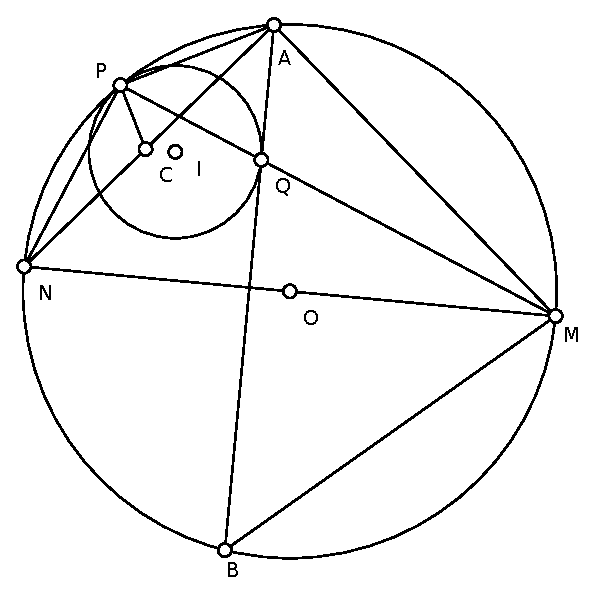
\includegraphics[width=\textwidth]{China2012.eps}
    \caption{}\label{fig:p4}
    \end{subfigure}~
    \begin{subfigure}[b]{0.45\textwidth}
    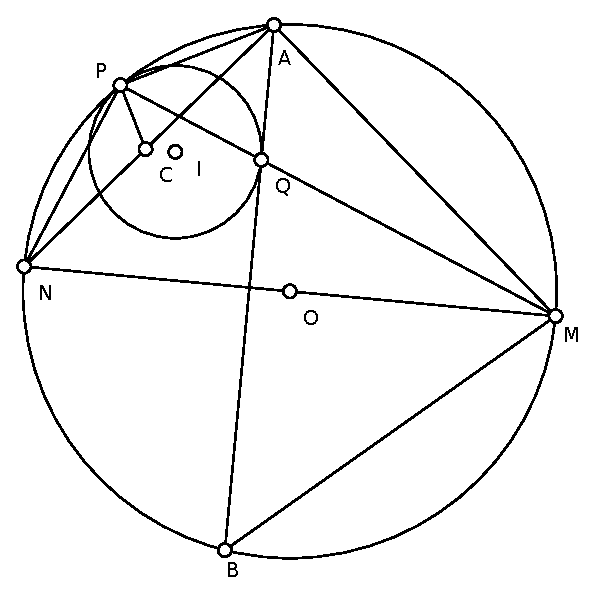
\includegraphics[width=\textwidth]{China2012.eps}
    \caption{}
    \end{subfigure}
    \caption{}
    \end{figure}


\item (2013年,30分) $AB$是圆$\omega$的一条弦,$P$为弧$AB$内的一点,$E,F$为线段$AB$上的两点,
满足$AE=EF=FB$。连接$PE,PF$并延长,与圆$\omega$分别交于点$C,D$,求证:
\[
EF\cdot CD = AC\cdot BD
\]

    \begin{figure}[!ht]
    \centering
    \begin{subfigure}[b]{0.45\textwidth}
    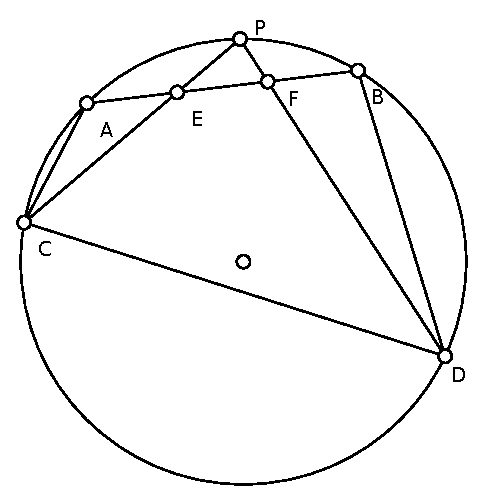
\includegraphics[width=\textwidth]{China2013.eps}
    \caption{}\label{fig:p5}
    \end{subfigure}~
    \begin{subfigure}[b]{0.45\textwidth}
    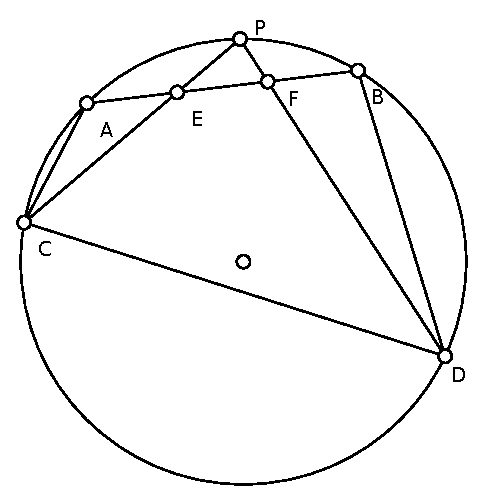
\includegraphics[width=\textwidth]{China2013.eps}
    \caption{}
    \end{subfigure}
    \caption{}
    \end{figure}
\item (2014年,40分) 
如图\ref{fig:China2014},在锐角三角形$ABC$中,$\angle BAC \neq 60^{\circ}$, 过点$B,C$分别作$\triangle ABC$的外接圆的切线$BD,CE$, 且满足 $BD=CE=BC$。直线$DE$与$AB,AC$的延长线分别交于点$F,G$. 设$CF$与$BD$交于点$M$,$CE$与$BG$交于点$N$。 证明:$AM=AN$。

    \begin{figure}[!ht]
    \centering
    \begin{subfigure}[b]{0.45\textwidth}
    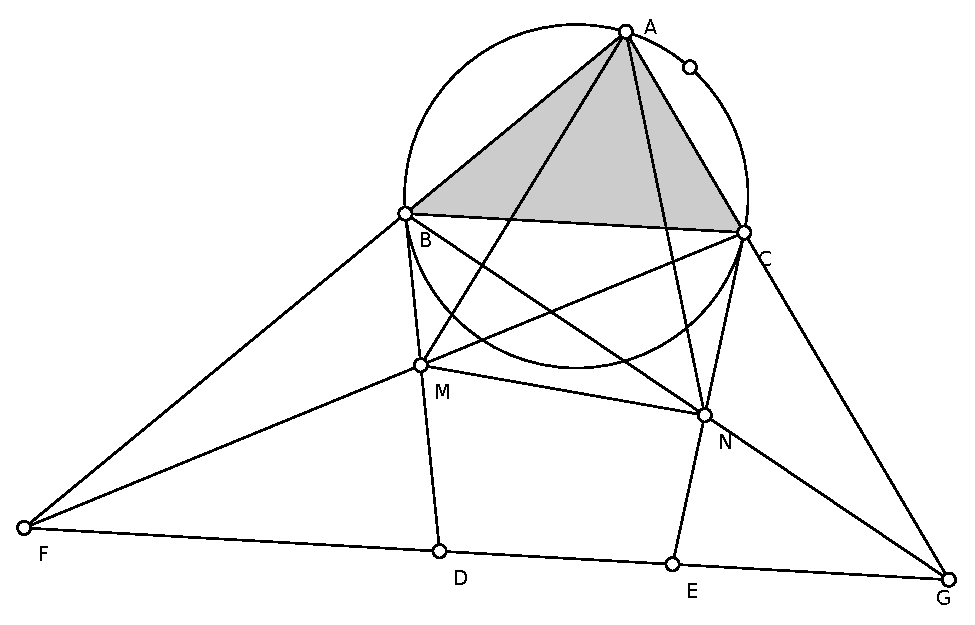
\includegraphics[width=\textwidth]{China2014.eps}
    \caption{}\label{fig:China2014}
    \end{subfigure}~
    \begin{subfigure}[b]{0.45\textwidth}
    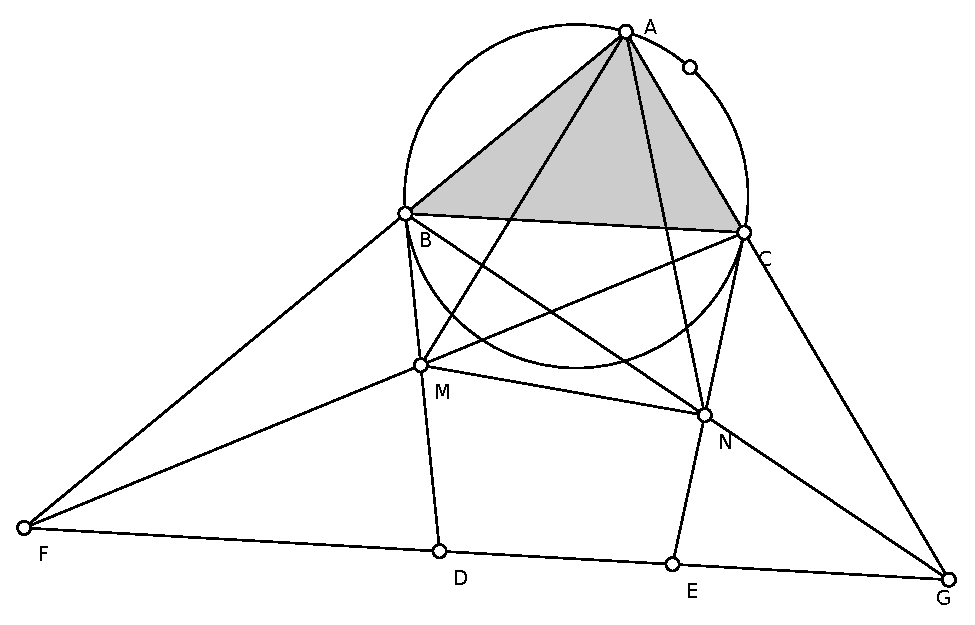
\includegraphics[width=\textwidth]{China2014.eps}
    \caption{}
    \end{subfigure}
    \caption{}
    \end{figure}

\item (2015年,50分) 如图\ref{fig:China2015},$\triangle ABC$内接于圆$O$,$P$为
$\widearc{BC}$ 上一点,点$K$在线段$AP$上,使得$BK$平分$\angle ABC$,过$K,P,C$三点的圆$\Omega$与边
$AC$交于点$D$,连接$BD$交圆$\Omega$于点$E$,连接$PE$并延长与边$AB$交于点$F$。证明:$\angle ABC=2\angle FCB$。

    \begin{figure}[!ht]
    \centering
    \begin{subfigure}[b]{0.45\textwidth}
    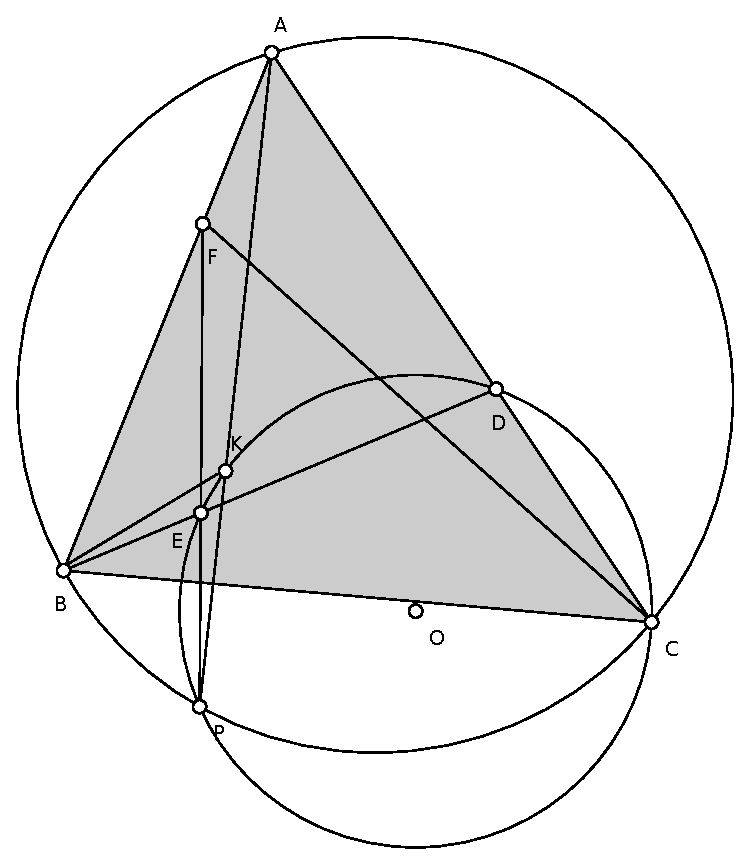
\includegraphics[width=\textwidth]{China2015.eps}
    \caption{}\label{fig:China2015}
    \end{subfigure}~
    \begin{subfigure}[b]{0.45\textwidth}
    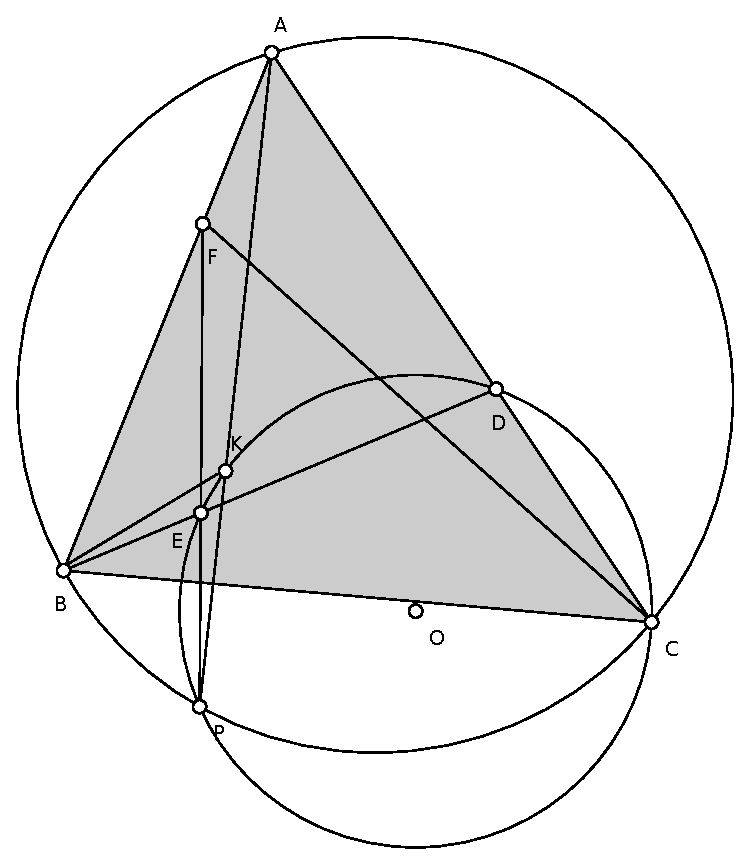
\includegraphics[width=\textwidth]{China2015.eps}
    \caption{}
    \end{subfigure}
    \caption{}
    \end{figure}

\item (2016年,40分) 如图\ref{fig:China2016},在$\triangle ABC$中, $X,Y$是直线上两点$(X,B,C,Y)$
顺序排列,使得$BX\cdot AC =CY\cdot AB$。 设$\triangle ACX,\triangle ABY$的外心分别为$O_1,O_2$,直线$O_1O_2$与
$AB,AC$分别交于点$U,V$。证明:$\triangle AUV$是等腰三角形。

    \begin{figure}[!ht]
    \centering
    \begin{subfigure}[b]{0.45\textwidth}
    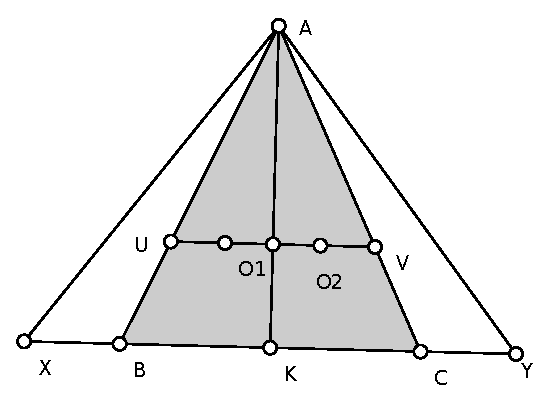
\includegraphics[width=\textwidth]{China2016.eps}
    \caption{}\label{fig:China2016}
    \end{subfigure}~
    \begin{subfigure}[b]{0.45\textwidth}
    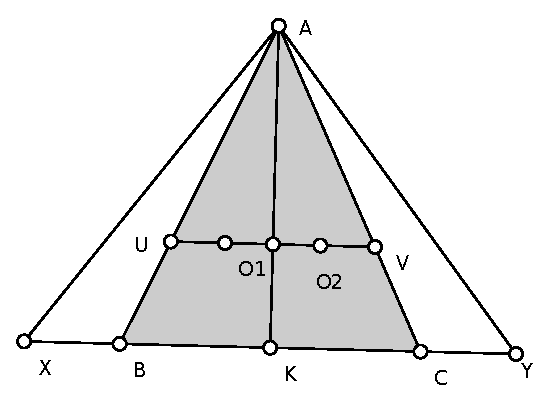
\includegraphics[width=\textwidth]{China2016.eps}
    \caption{}
    \end{subfigure}
    \caption{}
    \end{figure}
   

\item (2017年A卷,40分) 如图\ref{fig:China20172},在$\triangle ABC$中,$AB=AC$,$I$为$\triangle ABC$的内心,以$A$为圆心,$AB$为半径作圆$\Gamma_1$;以$I$为圆心,$IB$为半径作圆$\Gamma_2$,过点$B,I$的圆$\Gamma_3$与$\Gamma_1,\Gamma_2$分别交于点$P,Q$(不同于点$B$),设$IP$与$BQ$交于点$R$。证明:$BR\perp CR$。

    \begin{figure}[!ht]
    \centering
    \begin{subfigure}[b]{0.45\textwidth}
    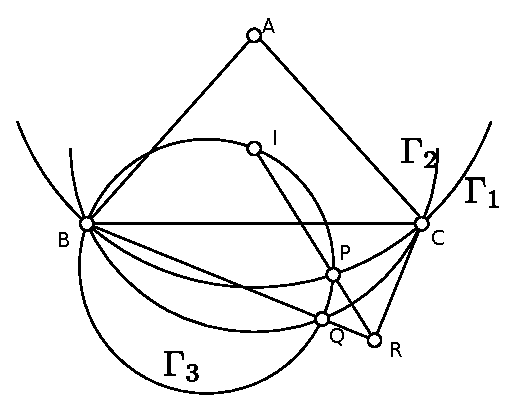
\includegraphics[width=\textwidth]{China20172.eps}
    \caption{}\label{fig:China20172}
    \end{subfigure}~
    \begin{subfigure}[b]{0.45\textwidth}
    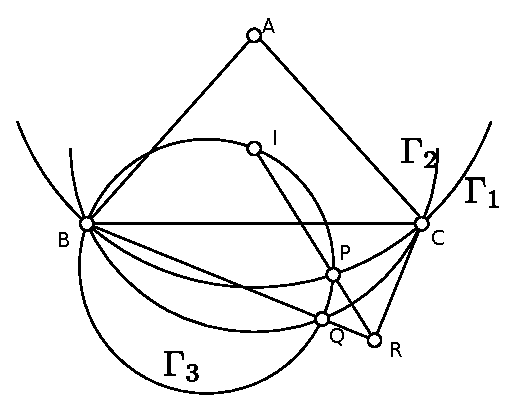
\includegraphics[width=\textwidth]{China20172.eps}
    \caption{}
    \end{subfigure}
    \caption{}
    \end{figure}
   

\item (2017年B卷,50分) 如图\ref{fig:China2017},点$D$是锐角$\triangle ABC$的外接圆$\omega$上弧$BC$
的中点,直线$DA$与圆$\omega$过点$B,C$的切线分别相交于点$P,Q$,$BQ$与$AC$的交点为$X$,$CP$与$AB$的交点为$Y$,$BQ$与$CP$的交点为$T$,求证:$AT$平分线段$XY$。

    \begin{figure}[!ht]
    \centering
    \begin{subfigure}[b]{0.45\textwidth}
    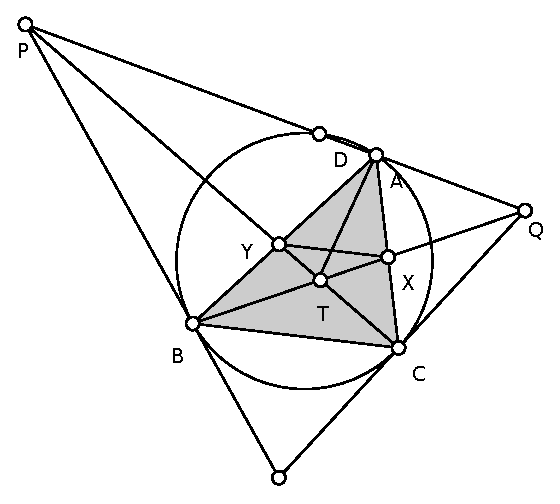
\includegraphics[width=\textwidth]{China2017.eps}
    \caption{}\label{fig:China2017}
    \end{subfigure}~
    \begin{subfigure}[b]{0.45\textwidth}
    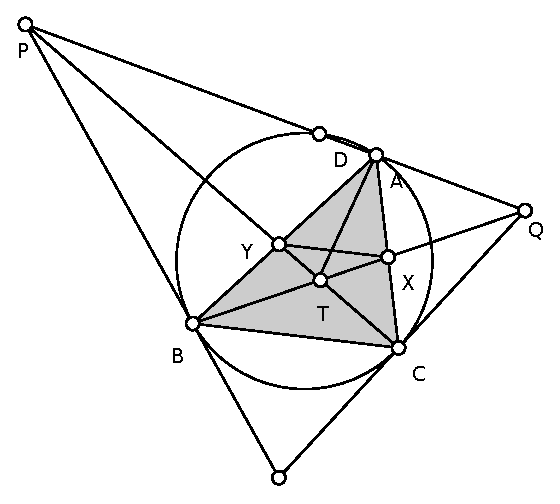
\includegraphics[width=\textwidth]{China2017.eps}
    \caption{}
    \end{subfigure}
    \caption{}
    \end{figure}

\end{enumerate}

\end{document}
cd
